\documentclass{beamer}
\usepackage{listings}
\usepackage{graphicx}
%\tcbset{
%texexp/.style={
%fonttitle=\small\sffamily\bfseries, fontupper=\small, fontlower=\small},
%example/.code 2 args={\refstepcounter{texexp}\label{#2}%
%    \pgfkeysalso{texexp,title={Listing \thetexexp: #1}}},
%}

%Define Colors
\definecolor{gray}{RGB}{102,102,102}		%#666666
\definecolor{lightblue}{RGB}{0,102,153}		%#006699
\definecolor{lightgreen}{RGB}{102,153,0}	%#669900
\definecolor{bluegreen}{RGB}{51,153,126}	%#33997e
\definecolor{magenta}{RGB}{217,74,122}		%#d94a7a
\definecolor{orange}{RGB}{226,102,26}		%#e2661a
\definecolor{purple}{RGB}{181, 0, 209}		%#7d4793
\definecolor{green}{RGB}{113,138,98}		%#718a62

% solarized https://en.wikipedia.org/wiki/Solarized
\definecolor{sblue}{RGB}{38,139,210}
\definecolor{syellow}{RGB}{181,137,0}
\definecolor{sgreen}{RGB}{113,163,0}
\definecolor{sviolet}{RGB}{108,113,196}


\lstdefinelanguage{ispc}{
  %Types
  morekeywords = [1]{int16, int32, int64, uint, uint16, uint32, uint64, int8, uint8, void, int, float, double, float16, int64\_t, int32\_t, char, uint32\_t, memblock, futhark\_context, free\_struct, fs\_struct, mem\_struct, my\_struct *},
  %Control flow
  morekeywords = [2]{catch, do, for, if, else, switch, while, foreach, foreach\_active, cif, return},
  %Qualifiers and stuff
  morekeywords = [3]{uniform, varying, export, extern, struct, unmasked, static, inline, unsigned},
  % Remaining functions
  morekeywords = [4]{extract, insert, reduce\_add, programIndex, programCount, reduce\_op, bin\_op, scan\_op, map\_op},
  keywordstyle = [1]\color{syellow}\bfseries,
  keywordstyle = [2]\color{sgreen}\bfseries,
  keywordstyle = [3]\color{sblue}\bfseries,
  keywordstyle = [4]\color{sviolet}\bfseries,
  sensitive = true,
  morecomment = [l]{//},
  morecomment = [s]{/*}{*/},
  morecomment = [s]{/**}{*/},
  commentstyle = \color{gray},
  morestring = [b]",
  morestring = [b]',
  stringstyle = \color{orange}
}

\lstdefinelanguage{futhark}{
  %Types
  morekeywords = [1]{f32, f64, i32, i64, void, int, float, double, float16, int64\_t, int32\_t, char, uint32\_t, memblock, futhark\_context, free\_struct, fs\_struct, mem\_struct, my\_struct *},
  %Control flow
  morekeywords = [2]{loop, let, def, catch, do, for, if, else, switch, while, foreach, foreach\_active, cif, return},
  %Qualifiers and stuff
  morekeywords = [3]{map, scan, reduce, reduce_by_index, uniform, varying, export, extern, struct, unmasked, static, inline, unsigned},
  % Remaining functions
  morekeywords = [4]{extract, insert, reduce\_add, programIndex, programCount, reduce\_op, bin\_op, scan\_op, map\_op},
  keywordstyle = [1]\color{syellow}\bfseries,
  keywordstyle = [2]\color{sgreen}\bfseries,
  keywordstyle = [3]\color{sblue}\bfseries,
  keywordstyle = [4]\color{sviolet}\bfseries,
  sensitive = true,
  morecomment = [l]{//},
  morecomment = [l]{--},
  morecomment = [s]{/*}{*/},
  morecomment = [s]{/**}{*/},
  commentstyle = \color{gray},
  morestring = [b]",
  morestring = [b]',
  stringstyle = \color{orange}
}

\usepackage{courier}

\lstset{
  basicstyle={\ttfamily\footnotesize},
  identifierstyle={\ttfamily},
  commentstyle={\itshape\ttfamily},
  keywordstyle={\bfseries},
  ndkeywordstyle={\bfseries},
  stringstyle={\ttfamily},
  breaklines=true,
  %columns=[l]{fullflexible},
  xrightmargin=0em,
  xleftmargin=2mm,
  numberstyle={\scriptsize},
  stepnumber=1,
  numbersep=1em,
  lineskip=-0.5ex,
  tabsize=4
}


\usetheme{Madrid}
\usecolortheme{beaver}

\title{Bachelor forsvar}
\subtitle{Udnyttelse af ISPC på Futharks multicore backend}
\author{Kristoffer A. Kortbaek}
\date{23. juni 2022}

%%Front page
\begin{document}
\begin{frame}
  \titlepage
\end{frame}

%% Slide 0
\begin{frame}
  \frametitle{Udnyttelse af language C-quote}
\end{frame}

%%Slide 1
\begin{frame}[fragile]
  \frametitle{Multicore flattening - sekventielle og parallelle SOACs}
  Når en SOAC har nested parallelisme, og dermed indeholder indre SOACs, så genereres to versioner
  \begin{enumerate}
    \item{Hver indre SOAC er blevet sekventialiseret}
    \item{De indre SOACs er uberørte og kører i parallel på flere kerner}
  \end{enumerate}

  \begin{lstlisting}[language=futhark]
    def main m n  (X:[m][n]i32)  (v:[n]i32)  =
      map (\x ->
        reduce (+) 0 (map2 (*) x v)
      ) X
    \end{lstlisting}
    Hvis den ydre \texttt{map} indeholder flere iterationer end antal logiske kerner på CPUen sekventialiseres \texttt{reduce}

  \end{frame}

\begin{frame}[fragile]
  \begin{itemize}
  \item Sekventialiseret
    \begin{lstlisting}[language=ispc]
        for(int map_i = 0; i < map_end; map_i++) {
          int red_res = 0; //Neutral element
          for(int red_i = 0;  red_end; red_i++) {
            int x = mem[map_i * n + red_i];
            int v_i = mem[red_i];
            int mul_res = x * v_i;
            red_res = mulres + red_res;
          }
          mem[map_i] = red_res;
        }
      \end{lstlisting}
    \item Parallel nested \texttt{reduce}
      \begin{lstlisting}[language=ispc]
        //map
        for(int map_i = 0; i < map_end; map_i++) {
          // schedule work for the nested reduce
          mem[map_i] = reduce_res;
        }
        //reduce
        for(int red_i = 0;  red_end; red_i++) {
          int x = mem[map_i * n + red_i];
          int v_i = mem[red_i];
          int mul_res = x * v_i;
          red_res = mulres + red_res;
        }
      \end{lstlisting}

  \end{itemize}

\end{frame}

%% Slide 2
\begin{frame}
  \frametitle{Vektoriseret \texttt{reduce}}
  \begin{enumerate}
  \item Begge versioner af en given SOAC kan tage gavn af data parallelisme
  \item Vi udvider ISPC i vores backend for at hver tråd udnytter data parallelisme
  \item Hver parallel SOAC i Futhark har en speciel vektoriseret algoritme
  \item Særligt har \texttt{reduce} fire forskellige kodegenereringer
    \begin{itemize}
    \item kommutative \texttt{reduce}
    \item normal(ikke kommutative) \texttt{reduce}
    \item \texttt{reduce} på en ``mapped'' operator
    \item Ingen brug af vektorisering
    \end{itemize}
  \end{enumerate}
\end{frame}

\begin{frame}[fragile]
  \frametitle{Kommutative reduktioner}
  \begin{block}{Kommutative reduktioner genereres der særligt effektiv kode for}
  \begin{enumerate}
    \item Den binære operator kan ske i vilkårlig rækkefølge: $a + b = b + a$
    \item Hver \textit{program instance} kan arbejde på sit eget segment af inputtet
  \end{enumerate}
  \end{block}
Givet et input array
\begin{figure}[h!]
  \centering
  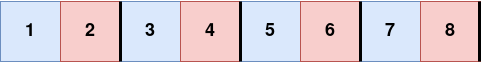
\includegraphics[width=0.5\textwidth]{input.png}
\end{figure}
  Kan vi ved en vectoriseret algoritme behandle den i tre trind
  \begin{columns}
    \column{0.5\textwidth}
  \begin{figure}[h!]
    \centering
    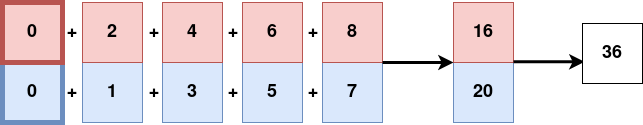
\includegraphics[width=0.7\textwidth]{kom_reduction.png}
  \end{figure}

  \column{0.4\textwidth}
  \begin{lstlisting}[language=futhark]
    reduce (+) 0 as
  \end{lstlisting}

  % \begin{align*}
  %   \texttt{reduce}: \hspace{0.5cm} &(\alpha \rightarrow \alpha \rightarrow \alpha) \rightarrow \alpha \rightarrow [n]\alpha \rightarrow \alpha
  % \end{align*}
  \end{columns}
\end{frame}
\begin{frame}[fragile]
  \frametitle{Kompileret program}
  \begin{lstlisting}[language=futhark]
    reduce (+) 0 as
  \end{lstlisting}
  Hver program instance kan lave siden egen reduktion.
  \begin{lstlisting}[language=ispc]
    int acc = 0;
    uniform int uni_acc = 0;
    foreach(Reduce_i = 0 ... n) {
      int a = mem[Reduce_i];
      int res = acc + a;
      acc = res;
    }
    foreach_active{i = 0 ... programCount} {
      uniform int a = extract(acc, i);
      uniformint res = uni_acc + a
      uni_acc = res;
    }
    mem_out[out] = uni_acc;
  \end{lstlisting}
  %Nævn der ikke er en garanti for rækkefølgen af program instansernes operatioenr

\end{frame}

\begin{frame}[fragile]
  \frametitle{Associative reduktioner}
  Rækkefølgen af den binære operator har betydning
\end{frame}

%% Slide 32
\begin{frame}
  \frametitle{Memory allocations}
\end{frame}

\end{document}
